
%(BEGIN_QUESTION)
% Copyright 2010, Tony R. Kuphaldt, released under the Creative Commons Attribution License (v 1.0)
% This means you may do almost anything with this work of mine, so long as you give me proper credit

Anta at en 12-bit DAC i et PLC analogt utgangskort har digitalt område 0 til 4095 counts (desimal) og analogt område 0 til 20 mA:

$$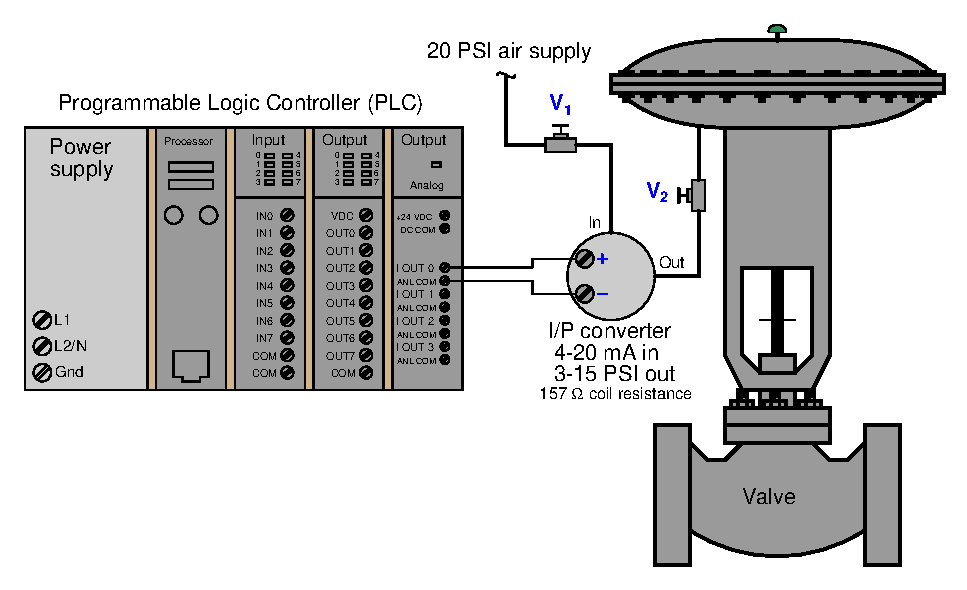
\includegraphics[width=15.5cm]{i00737x01.eps}$$

Anta at ventilspindel står på 5\% når kanalregisteret viser 604 counts (heksadesimal). En tekniker måler DC-spenningen over I/P-terminalene og får 1.18 volt.

\vskip 10pt

Beregn først korrekt ventilposisjon for denne registerverdien. Vurder deretter sannsynligheten for hver oppgitt feil. Ta én feil om gangen (ingen sammenfallende feil), og avgjør om hver feil alene kan forklare {\it alle} symptomer og målinger.

% No blank lines allowed between lines of an \halign structure!
% I use comments (%) instead, so that TeX doesn't choke.

$$\vbox{\offinterlineskip
\halign{\strut
\vrule \quad\hfil # \ \hfil &
\vrule \quad\hfil # \ \hfil &
\vrule \quad\hfil # \ \hfil \vrule \cr
\noalign{\hrule}
%
% First row
{\bf Feil} & {\bf Mulig} & {\bf Umulig} \cr
%
\noalign{\hrule}
%
% Another row
Brudd mellom ``I OUT 0'' og ``+'' terminal &  &  \cr
%
\noalign{\hrule}
%
% Another row
Brudd mellom ``ANL COM'' og ``$-$'' terminal &  &  \cr
%
\noalign{\hrule}
%
% Another row
I/P feilkalibrert &  &  \cr
%
\noalign{\hrule}
%
% Another row
Kortsluttet kabel mellom PLC og I/P &  &  \cr
%
\noalign{\hrule}
%
% Another row
Defekt analogutgangskort i PLC &  &  \cr
%
\noalign{\hrule}
%
% Another row
Ventil V1 stengt &  &  \cr
%
\noalign{\hrule}
%
% Another row
Ventil V2 stengt &  &  \cr
%
\noalign{\hrule}
%
% Another row
I/P-restriktor tett (helt/delvis) &  &  \cr
%
\noalign{\hrule}
%
% Another row
I/P-dyse tett (helt/delvis) &  &  \cr
%
\noalign{\hrule}
} % End of \halign
}$$ % End of \vbox

Til slutt: identifiser {\it neste} diagnostiske test/måling du ville gjort, og forklar hvordan resultatet avklarer feiltype/lokasjon videre.

\vfil

\underbar{file i00737}
\eject
%(END_QUESTION)





%(BEGIN_ANSWER)

Dette er en vurdert oppgave -- ingen svar eller hint er gitt!

%(END_ANSWER)





%(BEGIN_NOTES)

604 hex = 1540 desimal. Med fullskala 4095 counts tilsvarer dette 7.52 mA, altså litt under 25\% (nærmere bestemt 22\%). Siden ventilen står på 5\%, har vi et problem.

\vskip 10pt

1.18 V over I/P-motstand 157 ohm gir 7.52 mA, nøyaktig som forventet fra DAC-verdi. Dermed går riktig strøm til I/P, og PLC analogutgangen fungerer sannsynligvis. Mulige feil er da mekaniske/pneumatiske fra I/P og ut til ventilen.

% No blank lines allowed between lines of an \halign structure!
% I use comments (%) instead, so that TeX doesn't choke.

$$\vbox{\offinterlineskip
\halign{\strut
\vrule \quad\hfil # \ \hfil &
\vrule \quad\hfil # \ \hfil &
\vrule \quad\hfil # \ \hfil \vrule \cr
\noalign{\hrule}
%
% First row
{\bf Feil} & {\bf Mulig} & {\bf Umulig} \cr
%
\noalign{\hrule}
%
% Another row
Brudd mellom ``I OUT 0'' og ``+'' terminal &  & $\surd$ \cr
%
\noalign{\hrule}
%
% Another row
Brudd mellom ``ANL COM'' og ``$-$'' terminal &  & $\surd$ \cr
%
\noalign{\hrule}
%
% Another row
I/P feilkalibrert & $\surd$ &  \cr
%
\noalign{\hrule}
%
% Another row
Kortsluttet kabel mellom PLC og I/P &  & $\surd$ \cr
%
\noalign{\hrule}
%
% Another row
Defekt analogutgangskort i PLC &  & $\surd$ \cr
%
\noalign{\hrule}
%
% Another row
Ventil V1 stengt &  & $\surd$ \cr
%
\noalign{\hrule}
%
% Another row
Ventil V2 stengt & $\surd$ &  \cr
%
\noalign{\hrule}
%
% Another row
I/P-restriktor tett (helt/delvis) & $\surd$ &  \cr
%
\noalign{\hrule}
%
% Another row
I/P-dyse tett (helt/delvis) &  & $\surd$ \cr
%
\noalign{\hrule}
} % End of \halign
}$$ % End of \vbox

V1 kan ikke være helt stengt, for da ville ventilen ikke åpnet i det hele tatt. At den er 5\% åpen viser at noe lufttrykk faktisk når både I/P og aktuator.

\vskip 10pt

Et godt neste steg er å manuelt påvirke I/P flapper/dyse og forsøke å tvinge full utgang. Hvis ventilen da åpner fullt, er feilen trolig kalibrering eller mekanikk inne i I/P. Hvis ikke, kan V2 være stengt, I/P ha alvorlig feil, eller forsyningstrykket være for lavt.

%INDEX% Elektronikkrepetisjon: konvertering til/fra heksadesimal
%INDEX% Elektronikkrepetisjon: DAC-utgangsberegning

%(END_NOTES)
